	\chapter{Implementation}
	The goal of this chapter is to describe how the activities were implemented, regarding the hardware aspects, as well as the software ones.
	\section{Hardware platforms}
	{\textbf{\Large Dolphin Sam}} \newline \newline
	The main device used was Dolphin Sam, a smart object developed by I3Lab.
	[immagine delfino] \newline
	\noindent
	\textit{SAM FAI LA CITAZIONE SCHIAVO}Dolphin Sam is a stuffed toy enhanced with complex system made	up of several embedded sensors, actuators and external components. Four parts of the body, such as head, stomach, right and left fins are integrated with four touch sensors. There are light actuators on the stomach and a speaker and an RFID reader into the mouth. Eyes and mouth movements are controlled by two different motors. In addition a chip is used for Wi-Fi communication. \newline
	All embedded components are connected and managed by an Arduino module which manages also the communication between the smart dolphin and the external components, such as smart lights and tagged RFID cards.
	
	
	
	

		
	\section{Hardware architectures}
	The hardware architecture of the system is based on a three tier client-server architecture, where we can distinguish between:
	\begin{center}
		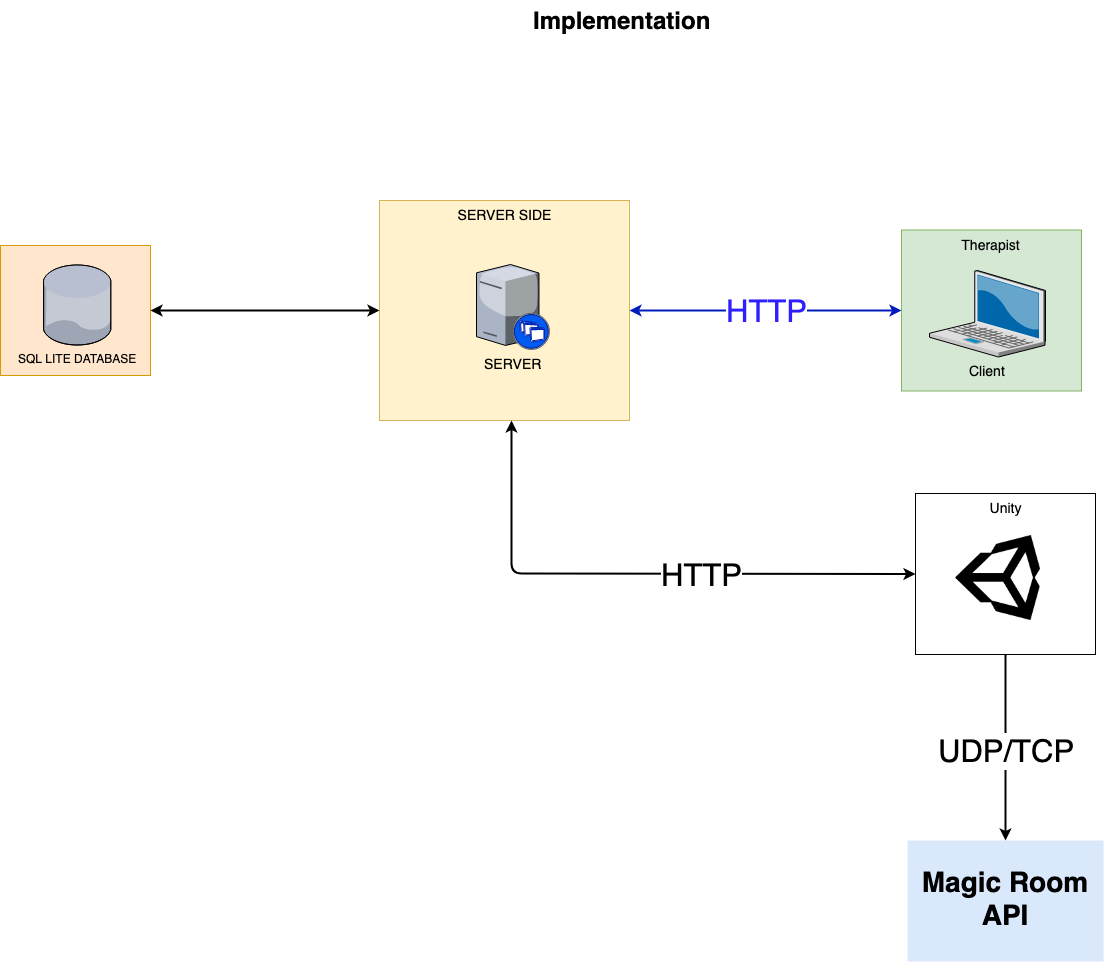
\includegraphics[width=\textwidth]{images/Architecture-Diagram.png}
	\end{center}
	\begin{itemize}
		\item \textbf{Data tier:} consists of a SQL Lite database
		\item \textbf{Application tier:} consists of a python flask web server which is built on REST architecture and contains part of the application logic. SQLAlchemy is used as Object Relational Mapper in order to query and manipulate data from the database, using an object-oriented paradigm.
		\item \textbf{Presentation tier:} represented the fron-end of our architecture, consists of web-based application accessible through a web-browser and three-dimensional games activities, built using Unity Game Engine platform, both communicating through HTTP calls with the server.
	\end{itemize}
	\noindent
	Unity game activities were implemented using a fat client approach by placing the whole application logic inside the presentation level. \newline
	Unity game engine uses the Magic Room API in order to interact with the smart object Dolphin Sam and with the external components inside the Magic Room such as kinect, smart lights and bubble machine.
	
	
	\section{Software Architectures}
	Regarding the server side, the software architecture was based on the \textbf{MVC} (Model View Controller) design pattern, where the main components are:
	\begin{itemize}
		\item \textbf{Controller:} responsible to dispatch all the requests coming from client side, both web application and unity game engine. The controller is also responsible to loads the views to display in the web application.
		\item \textbf{Model:} responsible for mapping user-defined python classes with database tables
		\item \textbf{View:} responsible for represent data coming from the model as user interface. HTML templates are used.
	\end{itemize}

	\noindent
	Regarding the software implementation of the game activities on client side, the software architecure was organized in three main modules:
	\begin{itemize}
		\item \textbf{Menu}
		\item \textbf{Run Activity}
		\item \textbf{Search Activity}
	\end{itemize}
	\noindent
	 that were treated separately. \newline
	 
	 Referring to Menu module, the main components are:
	 \begin{itemize}
	 	\item {Login Manager:} responsible for managing the login procedure and the communication with the server.
	 	\item {Menu Session Manager:} responsible for handling information coming from the server and for managing the user session
	 \end{itemize}
 
 	Referring to Run Activity module, the main components are:
 	\begin{itemize}
 		\item {Player Manager:} responsible for managing the player behaviour in the scene.
 		\item {Run Session Manager:} responsible for gathering information referring to the game session and dispatch those to the Menu Session Manager
 	\end{itemize}
 
 	Referring to Search Activity module, the main components are:
 	\begin{itemize}
 		\item {Player Manager:} responsible for managing the player behaviour in the scene.
 		\item {Search Session Manager:} responsible for gathering information referring to the game session and dispatch those to the Menu Session Manager
 	\end{itemize}
 
	\section{Programming languages and software used}
	The programming languages used ti develop the system are:
	\begin{itemize}
		\item C\#: Used for the realization of the Unity scripts.
		\item Python: Used for the server implementation
		\item HTML \& CSS: used for the realization of the web pages’ front-end.
		\item JavaScript: used for the realization of the web pages’ back-end.
	\end{itemize}
	\noindent
	The software that were used during the development are:
	\begin{itemize}
		\item Unity 2018.1.0f2 for the development of the game activities
		\item Visual Studio 2017 for the develoment of unity scripts.
		\item Intellij 2018.3 for the development of the server.
		\item SublimeText 3 for the development of the web pages.
		\item Git to synchronize the development between the members of the team.
	\end{itemize}
	
	
 	
	
	
	
	
		
		
		 
	
	
	
	
	

